\section{Bootstrap}\label{ch:bootstrap}

A second method for producing additional information from a limited dataset is to use the bootstrap method. It is performed by shaking up the data and plucking out random observations, while allowing for the same observation to be included multiple times, to create a new sample. The process can then be repeated as many times as needed until the desired amount of data becomes available. 

\subsection{Theory}

\iffalse
A good explanation https://stats.stackexchange.com/questions/26088/explaining-to-laypeople-why-bootstrapping-works
\fi

Bootstrapping works on the assumption that distribution parameters are transitive. Such that a random number generated by taking the mean of N samples from a dataset containing N samples, but allowing for replacement, will be equally valid as a random number generated from the original population.

As an example dataset X contains N observations from the original population $\theta$ we resample from X until a new dataset Y with N elements is created. Assuming $\theta$ follows a Gaussian distribution then the mean of Y is a random number generated from the distribution of X which is an estimate of the actual distribution of $\theta$ where each observation is generated from $\theta$. Therefore the mean of Y is an estimated observation from $\theta$.

Assuming we have sufficient data then the estimated distribution can be used for generating a new, more populated, data set without sacrificing much of the quality. As the observed distribution is an estimate of the population distribution, the resulting dataset will have a distribution which is an estimate of the observations.

\iffalse % Olaf: A second attempt at writing this section. Keeping it for review purposes.
Bootstrapping works by resampling the initial data with replacement, until a new data set has been created from the original. The new dataset will then contain a random sample of data with the same distribution as the original, allowing for some deviation in the parameters. By repeating this B times and averaging the distribution parameters over all B samples we get a better estimate of the original population as if we had gotten more observations.

As an example, assuming we have a normally distributed population of N elements then by taking a random resampling from that dataset until a new dataset, also containing N elements, is gained. The mean of that new dataset can then be seen as an estimated new observation from the original population. We then repeat this process B times and in the end we have a new data set of both resampled means and variances. Since both were generated using the original set of observations the set of resamples will also be normally distributed with a mean and variance close to the original population.
\fi

To give an example of how bootstrap creates samples, see Figure \ref{fig:bootstrapDrawWithReplacement}\footnote{\cite{James2013} p. 190}. In the figure random observations are drawn from the estimated population (Original Data(Z)) with replacement. The amount of observations drawn per sample is the same amount as the observations of the estimated population. This creates bins of observations ($Z^{*1}, Z^{*2},\ldots,Z^{*B}$), from the estimated population, from which mean of the data X and Y are both calculated. The result is bootstrap samples ($\hat\alpha^{*1}, \hat\alpha^{*2}, \ldots, \hat\alpha^{*B}$).

\begin{figure}[H]
	\centering
	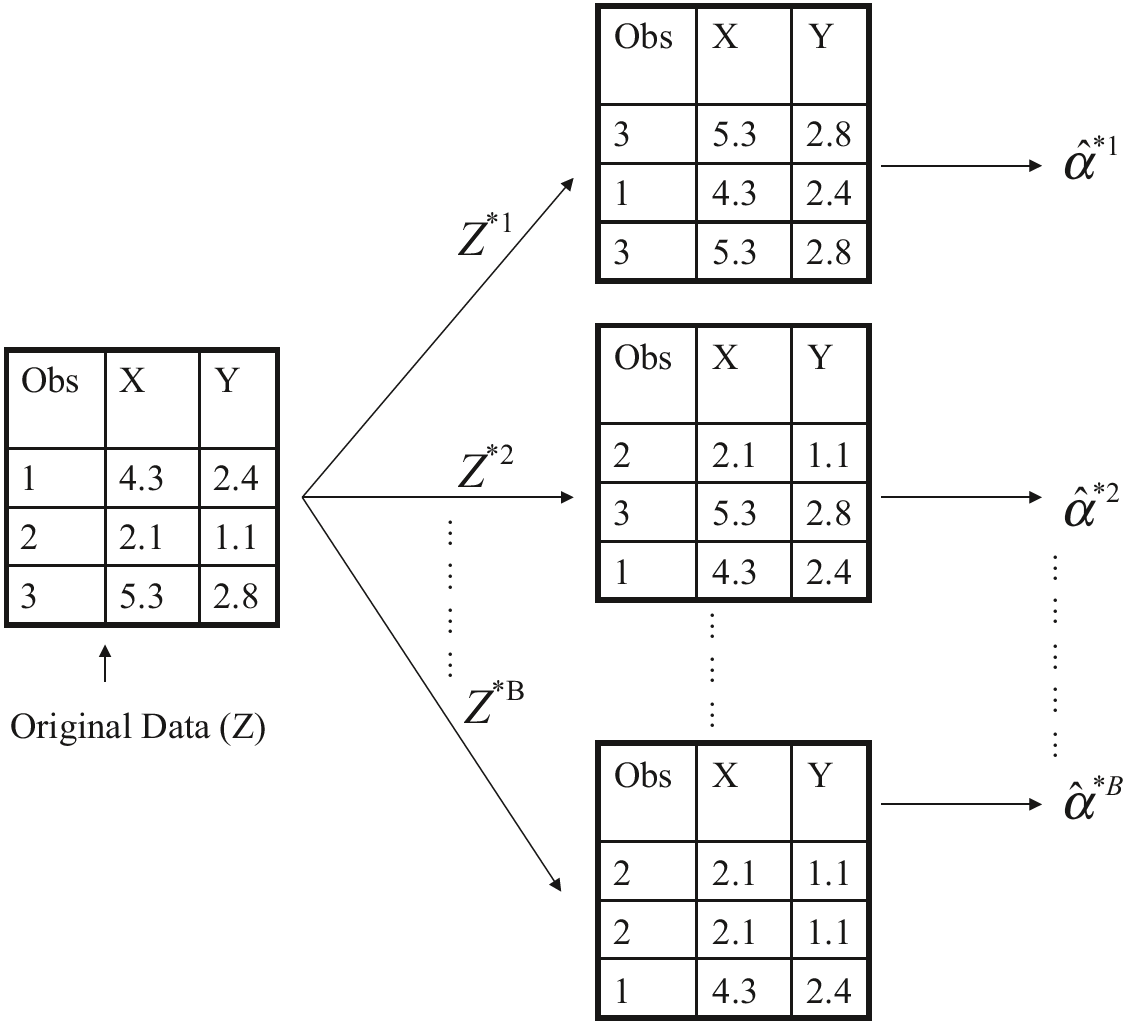
\includegraphics[width=0.5\linewidth]{crossValidation/bootstrapDrawWithReplacement}
	\caption{Bootstrap sample draw, with replacement.}
	\label{fig:bootstrapDrawWithReplacement}
\end{figure}

The standard error of the resampled data can be estimated through the sample standard deviation, as seen in Equation \ref{fo:bootstrapStandardError}. $\hat{\theta}$ denotes the bootstrap data of the estimated population $\theta$. $\hat{\theta_{b}}$ where $b=1,\dots,B$ denotes each bootstrap dataset. $\bar{\theta}$ denotes the mean of the bootstrap data; $\bar{\theta} = \frac{1}{B} \sum_{b=1}^{B}(\hat{\theta_{b}})$.
\begin{align}\label{fo:bootstrapStandardError}
	SE(\hat{\theta}) = \sqrt{\frac{1}{B-1} \sum_{b=1}^{B}(\hat{\theta_{b}} - \bar{\theta})} 
\end{align}

When working with more complex data, for example data that is not independent, but rather dependent on each other can create problems for the resampling methods of bootstrap. The solution to this problem is the Block Bootstrap alternative. Block Bootstrap does the same as the simple bootstrap mentioned earlier in this chapter, however before drawing samples from the estimated population, the data is put into smaller blocks, where the data is independent to each other. The block size is decided upon to maximize the amount of data that reside in a block, as well as minimizing the dependency between data in a single block.

\subsection{Results}
\subsubsection*{LAB 5.3.4}

In lab 5.3.4 on Bootstrap a small data sample is taken and the bootstrapping method is used to increase the data quality. First to examine the process on the Portfolio data set, and then apply the method to the auto data set and review the results for linear and quadratic regression compared to the original.

The resulting mean and error for the intercept and horsepower.
\begin{lstlisting}[language=Python]
original params
  Intercept:  mean:  39.9358610212
  Intercept:  error: 0.717498655555
  horsepower: mean:  -0.157844733354
  horsepower: error: 0.00644550051769
Bootstrapped params
  Intercept:  mean:  39.9805602832
  Intercept:  error: 0.0288069750935
  horsepower: mean:  -0.158352159577
  horsepower: error: 0.000244810973842
\end{lstlisting}

For the linear regression very similar means for both the Intercept and horsepower are found, while the RSE has dropped sharply for both the intercept and horsepower. This shows that the original estimates of the parameters were quite good as most of the error in the estimate can be explained by noise in the data and not $\epsilon_i$ as the regression formula assumes.

For the end of the exercise the same code will be run, but using a quadratic term. This time the fit to the data is very good and we see similar results as the error drops by a factor of $\sim30$.

\begin{lstlisting}[language=Python]
original params
 Intercept:  mean:               56.9000997021
 Intercept:  error:              1.80042680631
 horsepower: mean:               -0.466189629947
 horsepower: error:              0.0311246171196
 np.power(horsepower, 2): mean:  0.00123053610077
 np.power(horsepower, 2): error: 0.00012207586276
Bootstrapped params
 Intercept:  mean:               57.072651342
 Intercept:  error:              0.066630006277
 horsepower: mean:               -0.469465867184
 horsepower: error:              0.00106828698911
 np.power(horsepower, 2): mean:  0.00124365698568
 np.power(horsepower, 2): error: 3.87603834867e-06
\end{lstlisting}



